% !TEX encoding = UTF-8 Unicode
\documentclass[aodsor,preprint]{imsart}
\usepackage{amsthm,amsmath,amssymb}
\usepackage{graphicx}
%\usepackage[authoryear,round]{natbib}
\usepackage[
backend=biber,
natbib=true,
language = english,
doi = false, url = false, isbn = false, eprint = false,
style = apa]
{biblatex}
\DeclareLanguageMapping{english}{english-apa}
\addbibresource{sources.bib}
\usepackage[colorlinks,citecolor=blue,urlcolor=blue]{hyperref}
\usepackage[utf8]{inputenc}
\usepackage{relsize}
\usepackage{dsfont}
\usepackage{float}
\usepackage{hyperref}
\usepackage{xcolor}
\usepackage{algorithm2e}
\usepackage{bm}
\usepackage{mathtools}
\usepackage{amsmath}
%\usepackage{algorithm}
%\usepackage{algpseudocode}
%\usepackage{ngerman}


% settings
%\pubyear{2005}
%\volume{0}
%\issue{0}
%\firstpage{1}
%\lastpage{8}
%\arxiv{arXiv:0000.0000}


\numberwithin{equation}{section}
\theoremstyle{plain}
\newtheorem{thm}{Theorem}[section]
\newtheorem{lemma}[thm]{Lemma}
\newtheorem{corollary}[thm]{Corollary}
\newtheorem{remark}[thm]{Remark}
\newtheorem*{remark*}{Remark}

% customize math operators
\newcommand{\E}{{\mathbb E}}
\DeclareMathOperator*{\argminA}{arg\,min}

\begin{document}

\begin{frontmatter}
\title{Scraping the Synthetic Risk and Reward Indicator from Funds' Key Information Documents}
\runtitle{Scraping Key Information Documents}

\begin{aug}
\author{\fnms{Fabian} \snm{Blasch}\ead[label=e1]{blasch57@gmail.com}}



\runauthor{Fabian Blasch}

\affiliation{University of Vienna}

\end{aug}

\begin{abstract}
The main objective of this paper is to extract the SRRI (Synthetic Risk and Reward Indicator) from funds' KIDs (Key Information Documents). Two approaches are presented, the naive approach which does not rely on any statistical methods and the clustering approach, which utilizes hierarchical agglomerative clustering. The naive approach manages to correctly predict 80\% of the test cases while the clustering approach performs worse at an accuracy of 70\%. Both methods do not generate any incorrectly predicted cases, i.e., the cases for which the SRRI is not scrapeable results in the applied function returning an error. 
\end{abstract}

\begin{keyword}[class=MSC]
\kwd[Primary ]{91C20}
\kwd{62H30}
%\kwd[; secondary ]{Key3}
\end{keyword}

\begin{keyword}
\kwd{Data Mining, Hierarchical Clustering}
\kwd{\LaTeXe}
\end{keyword}

\end{frontmatter}

\section{Introduction}
According to BGBl. II Nr. 265/2011, effective 2011, every undertaking for collective investment in transferable securities (UCITS), has to publish a key information document \citep{BGB1}. Said document is supposed to inform potential and current investors about various characteristics of the investment fund at hand. Besides a short description of the investments as well as performance measured against a benchmark, this document also contains a synthetic risk- and reward indicator (SRRI). As the name suggests, the purpose of this indicator is to measure the risk and return associated with an investment in the respective fund. How the SRRI is derived depends on data availability and will be described in greater detail in a separate section. Independent of the exact procedure of derivation the underlying interpretation of risk is measured via the volatility of returns.\\
The aim of this thesis is to firstly, give a short and precise introduction into the calculation of the SRRI. Then the data is briefly presented and the approach to measuring extraction performance is discussed. The following sections' focus shifts to extracting the SRRI which is displayed as a graph, usually on the first page of every KID. In order to keep the structure as simple as possible the proccess is split into two parent functions which call a variety of helper functions. All functions are implemented in R, besides the base library, the use of further libraries is pointed out in the description of the individual functions \citep{base}.

\newpage

\section{SRRI}

The SRRI aims to measure risk via the volatility of weekly returns from the last 5 years, should weekly retuns be unobtainable, the calculation may be executed using montly returns. Accordingly, by ordinance the SRRI may be obtained as follows

\[
\sigma_f = \sqrt{\frac{m}{T - 1}\text{ }\mathlarger{\sum}_{t = 1}^{T} (r_{f, t} - \overline{r_f})^2},
\]

where $r_{f, t}$ is the fund's return and $\overline{r_f}$ represents the mean of returns over $T$ periods. Then scaling via $m$, the return frequency within a year, yields the standard deviation of yearly returns. For illustrative purposes, the calculation using weekly returns would result in $m = 52$, as there are 52 weeks in a year and thus $T = 5 * 52 = 260$ represents the number of weeks in 5 years. To obtain the SRRI which is measured on a scale from 1 to 7 the regulating autorithy provides a table \citep{BGB1}.
\begin{table}[H]
\begin{center}
	\caption{SRRI Classification}
\begin{tabular}{|c|c|c}
	\hline
	SRRI & $\sigma_f$ \\
	\hline
	1 & $0\% \leq\sigma_f<0.5\%$\\
	\hline
	2 & $0.5\%\leq\sigma_f<2\%$\\
	\hline
	3 & $2\%\leq\sigma_f<5\%$\\
	\hline
	4 & $5\%\leq\sigma_f<10\%$\\
	\hline
	5 & $10\%\leq\sigma_f<15\%$\\
	\hline
	6 & $15\%\leq\sigma_f<25\%$\\
	\hline
	7 & $25\%\geq\sigma_f$\\
	\hline
\end{tabular}
\end{center}
\end{table}

\section{Measuring Scraping Performance}

The SRRI is measured on an increasing ordinal scale, with 7 being associated with the highest risk and simultaneously also with the highest return. This would in theory allow for a measurement of predictive performance utilizing the abolute or squared difference between prediction and actual value. However, in this case we want to measure whether the read-out was successful or not. Hence the performance evaluation will be based on predicting correctly. Formally this means, we will use a discrete metric, i.e., 

\[
Accuracy = \frac{1}{n}\mathlarger{\sum}_{i = 1}^n\mathds{1}_{\{pred_i \text{ }= \text{ } act_i\}}\text{.}
\]

Put differently, the accuracy measure is equivalent to the relative amount of correctly predicted cases.
\newpage

\section{Data}
The KIDs are available to download from the respective fund managing firm's website. The  sample contains 110 Key Information Documents, and can be found \href{https://github.com/Base-R-Best-R/KID/tree/main/KIDs}{\textcolor{teal}{here}}. First ten Kapitalanlagegesellschaften (KAG) that manage funds registered in austria were chosen.Then the sample was generated via randomly choosing funds on the respective websites of the fund managing firm. The distribution of the SRRI as well as the amount of KIDs per KAG within the sample are displayed below. Further, to obtain a test set, a stratified sampling proccess was applied, for each KAG two KIDs were randomly chosen. Accordingly, the training set used to optimize function input parameters includes 90 files while the test set contains 20 files. The code to generate the test set may be found \href{https://github.com/Base-R-Best-R/KID/blob/main/Code/Package/DEV/Generate_Test_Sample.R}{\textcolor{teal}{here}}. The rationale behind stratified sampling is that the sample is already quite small, random sampling across all files could thus poorly reflect the true document population. Moreover, for one of the functions applied, a color has to be passed as an argument, hence the stratified sampling allows to determine the color that is passsed via the file location which drastically reduces KAG identification effort for the document at hand. 

\begin{figure}[H]
	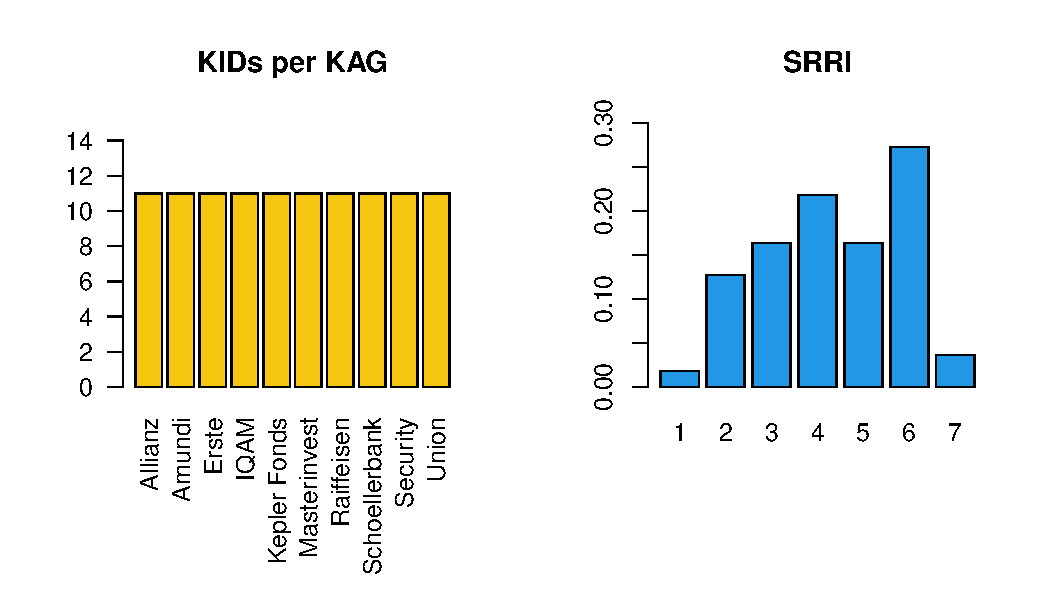
\includegraphics[width = 12cm]{data_overview.pdf}
	\caption{Number of KIDs per KAG and distribution of the SRRI}
\end{figure}

The two depicted plots provide a good summary of the sample at hand. We can immediately observe that for all fund managing firms, 11 KIDs are available in the sample. Regarding the distribution of the SRRI, the graph depicted on the right enables us to notice that the sample seems to contain very little funds that are associated with an SRRI of 1 or 7. The low number of funds classified into the first class may be due to the way the standard deviation of returns is converted into the SRRI. The intervals which are used to determin the SRRI differ in length quite significantly. The first interval for which $0\% \leq\sigma_f<0.5\%$ spans a range of half a percent, while the intervall for the classification into the 6th class $15\%\leq\sigma_f<25\%$ spans 10\%. The other end, namely the SRRI of 7, could be underrepresented because of a lack in demand for such high risk/return products. Of course, this is just mere speculation but interesting nonetheless.
In regards to the extraction, to ease illustration of the coming chapters, an example document from Erste can be found \href{https://github.com/Base-R-Best-R/KID/blob/main/KIDs/Erste/kid-eb-147-t2957-at_de-de_en_4.pdf}{\textcolor{teal}{here}}. Additionally, an example of the SRRI graph as it can be found in an Erste KID is provided below.

\begin{figure}[H]
	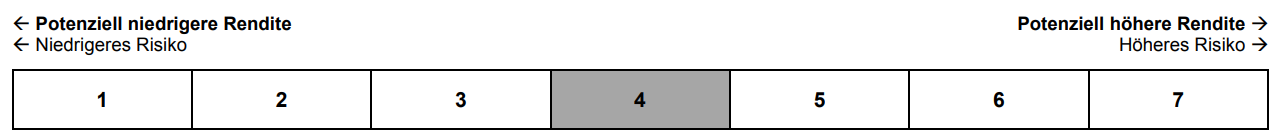
\includegraphics[width = 12cm]{example_SRRI_graph}
	\caption{Example of the SRRI graph from an Erste KID}
\end{figure}


\section{Extraction}

\subsection{Helper Functions}
Before splitting into the two approaches taken to obtain the SRRI, the helper functions that are utilized in both cases have to be explained. The naive approach relies on knowledge of the background color of the file at hand. In order to obtain this color, one can either assume that it is white, i.e., the color identification code being \href{https://www.color-hex.com/color/ffffff}{\textcolor{teal}{\#ffffffff}} or extract the most common color in the pdf. Both options are implemented, since obtaining the background color is a computationally intensive operation. The function called  \href{https://github.com/Base-R-Best-R/KID/blob/main/Code/Package/KIDs/R/bg_col.R}{\textcolor{teal}{bg\_col()}} first converts the input pdf file into a bitmap utilizing the R package pdftools \citep{pdftools}. A bitmap is an array of dimension $n \times m \times 4$, where $n$ and $m$ can be interpreted as the vertical and horizontal coordinates respectively while 4 signifies that each color entry is split into four substrings, the so called Hex code of the color. Hex which stands for hexadecimal would usually imply a string of six characters. However, in the case of inclusion of an alpha value the string includes 8 characters. The alpha value is used to alter the transparency of the color. An example for illustrative purposes, should we be interested in the color of the pixel that lies the furthest to the left on the top of the page we would subset with $n = 1$ and $m = 1$ to obtain the four substrings containing two characters each. Those 4 substrings then represent the color of the pixel. In order to obtain the background color, i.e., the most common color in the document we thus first flatten the array to an $n\times m$ matrix by pasting together the substrings of the Hex code to then find the color with the most entries in the matrix.\\
Besides the backgroundcolor, it is also important to localize the SRRI scale on the page, this task is designated to \href{https://github.com/Base-R-Best-R/KID/blob/main/Code/Package/KIDs/R/coord_id.R}{\textcolor{teal}{coord\_id()}}, which calls two additional helper functions. As each document contains many numbers, to identify which of those make up the SRRI graph, \href{https://github.com/Base-R-Best-R/KID/blob/main/Code/Package/KIDs/R/scale_cand_coord.R}{\textcolor{teal}{scale\_cand\_cord()}} first identifies which single digit numbers could possibly be part of the SRRI \citep{pdftools}. This is achieved by extracting all single digit numbers between 1 and 7 from the document, including the vertical and horizontal position on the page. Summarized in a matrix, this information is then passed to \href{https://github.com/Base-R-Best-R/KID/blob/main/Code/Package/KIDs/R/coord_id.R}{\textcolor{teal}{coord\_id()}}, which first finds the absolute difference in vertical/horizontal position of all candidates utilizing \href{https://github.com/Base-R-Best-R/KID/blob/main/Code/Package/KIDs/R/abs_dis_vec.R}{\textcolor{teal}{abs\_dis\_vec()}}, including some tolerance level, to then check if there exist 7 single digit entries with the same vertical/horizontal position. If this is the case, the function has succesfully identified the position of the SRRI. Accordingly, the function then returns a matrix containing the vertical and horizontal position of each scale entry as well as a string specifying whether the SRRI is displayed vertically or horizontally. Even though not a single occurance of a vertical SRRI depiction is included in the random sample of KIDs, this feature was implemented for the sake of completeness.

\subsection{Naive Approach}
To establish a benchmark for the extraction performance, the naive approach, as the name might suggest, does not make use of any statistical methods. The function \href{https://github.com/Base-R-Best-R/KID/blob/main/Code/Package/KIDs/R/SRRI_ext_rec.R}{\textcolor{teal}{SRRI\_ext\_rec()}} first localizes each of the 7 SRRI entries on the page via \href{https://github.com/Base-R-Best-R/KID/blob/main/Code/Package/KIDs/R/coord_id.R}{\textcolor{teal}{coord\_id()}}. Then the rectangles as displayed in blue in the figure below are built using vertical (yellow) and horizontal (red) tolerances measured from the location of each SRRI entry. Those tolerances are an argument of the function \href{https://github.com/Base-R-Best-R/KID/blob/main/Code/Package/KIDs/R/SRRI_ext_rec.R}{\textcolor{teal}{SRRI\_ext\_rec()}}, however, default values are implemented that achieve an accuracy of 100\% on all sample documents that are not scanned. Once the rectangles are built, the bitmap containing all color entries is subset to obtain the colors within the rectangle. Subsequently, the percentage of non-background colored pixels is calculated. Finally the rectangle with the least amount of background-colored pixels is choosen as the predicted SRRI.

\begin{figure}[H]
	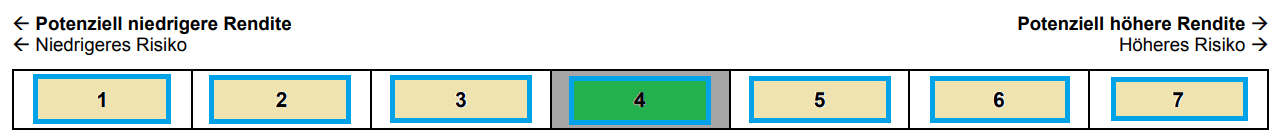
\includegraphics[width = 12cm]{example_SRRI_graph_naive}
	\caption{Illustration of the Naive Approach}
\end{figure}
\newpage
\subsection{Clustering Approach}
\subsubsection{Motivation}
The second approach is based on agglomerative hierarchical clustering. Before going into detail in regards to the technicalities of this clustering technique, firstly, the idea will be outlined using some graphical illustrations. Assume one knows the color that is used to shade the SRRI, in the case of figure 3 that would be grey (Hex: \href{https://www.color-hex.com/color/a6a6a6}{\textcolor{teal}{\#a6a6a6ff}}). Then an intuitive approach would be to subset all pixels in the color of the SRRI shade to then produce some sort of representative value of the horizontal location of the SRRI shade.

\begin{figure}[H]
	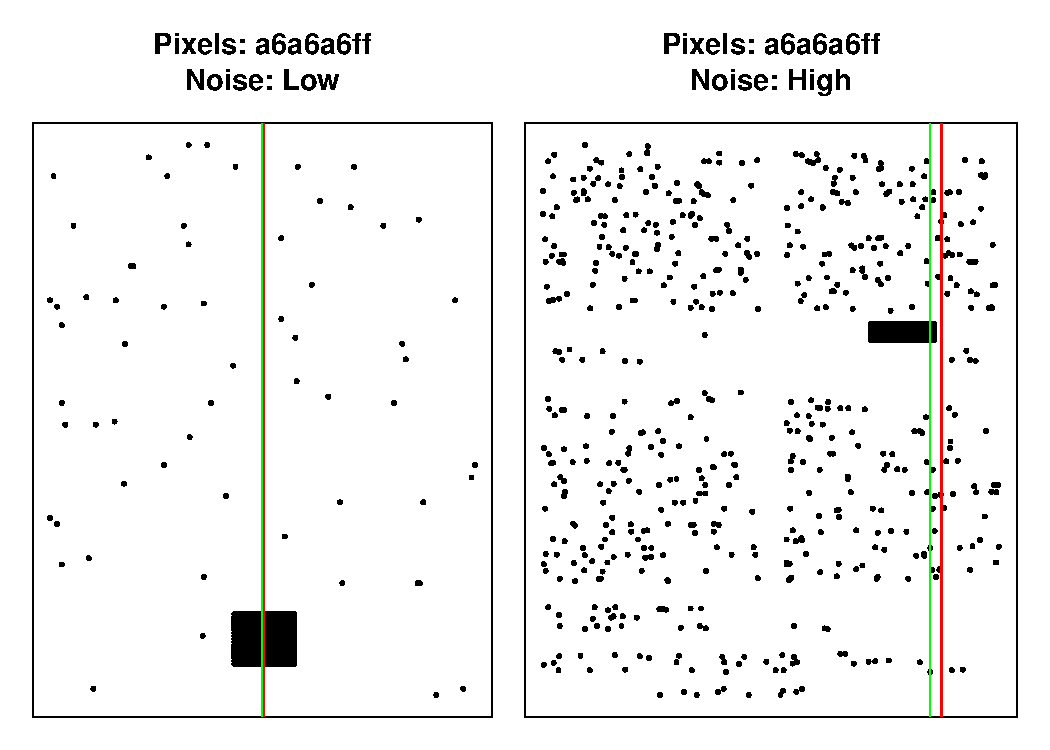
\includegraphics[width = 12cm]{highnoiselownoise.pdf}
	\caption{Pixels in the color of the SRRI shade}
\end{figure}

Above we observe the subset of pixels in the color of the SRRI shade for two different documents. Further, the mean of the horizontal coordinates of the pixels is represented by the green line while the median is represented by the red line. Unfortunately, this makes it painfully obvious that neither the median nor the mean of the horizontal coordinates will suffice as a representative of the cloud of pixels in the color of the SRRI shade. To be precise, the median is not a good representative, in a high noise enviroment as displayed on the right. Thus if we manage to reduce said noise to obtain a situation somewhat similar to the one on the left, we may be able to succesfully use the median as a good representative of the horizontal position of the SRRI pixel cloud. This noise reduction may be achieved via unsupervised classification into groups based on agglomerative hierarchical clustering.
\newpage
\subsubsection{Agglomerative Hierarchical Clustering}
The goal of noise reduction via clustering is achieved by grouping the pixels. The idea is to cluster the set of all pixels S into subsets $G_1, G_2,..., G_n$, such that the union of all groups $\cup_{i = 1}^n G_i$ forms a partition on the set of all pixels, i.e., $S = \cup_{i = 1}^n G_i$ where $G_i \cap G_j = \emptyset$ for $i \neq j$ \citep{Rok09}. Since the grouping is based on the similarity across pixel coordinates, we need a measure for similarity. In this thesis the euclidean distance is used to determine similarity.\\
The approach of agglomerative hierarchichal clustering starts by initially assigning each pixel its own cluster. Then in each iteration based on the minimal distance, clusters are merged until the desired number of clusters is obtained. In accordance with \citet{RPA2018} the algorithm may be denoted as follows:

\RestyleAlgo{ruled}

%% This is needed if you want to add comments in
%% your algorithm with \Comment
\SetKwComment{Comment}{/* }{ */}
% A distance matrix based on pairwise euclidean distance $\mathbf{D} \coloneqq Dist(G_i, G_j)\text{ }\forall\text{ }i, j$,\\
\begin{algorithm}[hbt!]
	\caption{\textit{Agglomerative Hierarchical Clustering}}\label{alg:one}
	\KwData{N vectors of pixel coordinates $\{x_i\}^N_{i = 1}$ and $p$ the number of desired clusters.}
	$\mathbf{X} \gets \emptyset$\ \Comment*[r]{Initialize empty set as storage for clusters}
	\For{$k \gets 1 ... N $}{ 
		$\mathbf{X} \gets \mathbf{X} \cup \{\{x_k\}\}$\Comment*[r]{Assign each pixels its own cluster}
	}
	$\mathbf{T} \gets \mathbf{X}$\Comment*[r]{Storage of clusters, to create a dendrogramm at a later stage}
	\While{$\lvert \mathbf{X} \rvert >  p$}{
		$G_1^*, G_2^* \gets  \underset{G_i, G_j \in \mathbf{X}}{\mathrm{argmin}} \text{ } Dist(G_i, G_j)\text{ } for \text{ } i \neq j$ \Comment*[r]{Find minimal distance}
		$\mathbf{X}  \gets (\mathbf{X}\setminus G_1^*)\setminus G_2^*$ \Comment*[r]{Remove individual occurances}
		$\mathbf{X} \gets \mathbf{X} \cup \{ G_1^* \cup  G_2^* \}$\Comment*[r]{Add union as new cluster}
		$\mathbf{T} \gets \mathbf{X} \cup \{ G_1^* \cup  G_2^* \}$;
	}
\end{algorithm}

Given that euclidean distance is used to judge similarity, the first iteration of the while loop is unambigous as only the distance between pixels is required for execution. However, starting from the second iteration we need to find the distance between pixels, other pixels and the first cluster. Hence, $Dist(G_i, G_j)$ needs to be defined for $G_i$ and/or $G_j$ as clusters. In this thesis three diffrernt approaches to determin the above described distance are considered.

\begin{enumerate}
	\item \textbf{Average-link:} $D(G_i, G_j) = D(\{x_k\}_{k = 1}^K, \{y_s\}_{s = 1}^S) = \frac{1}{KS} \mathlarger{\sum}_{k = 1}^K \mathlarger{\sum}_{s = 1}^S \lvert\lvert x_k - y_s\rvert \rvert$
	
	\item \textbf{Single-link:} $D(\{x_k\}_{k = 1}^K, \{y_s\}_{s = 1}^S) = \underset{k, s}{min} \lvert \lvert x_k - y_s\rvert \rvert$
	
	\item \textbf{Complete-link:}  $D(\{x_k\}_{k = 1}^K, \{y_s\}_{s = 1}^S) = \underset{k, s}{max} \lvert \lvert x_k - y_s\rvert \rvert$
\end{enumerate}

At a later stage the link will be chosen based on prediction accuracy. For illustrative purposes, the clustering for different links and varying numbers of final clusters is displayed.\newpage

%methodsclust.pdf
\begin{figure}[H]
	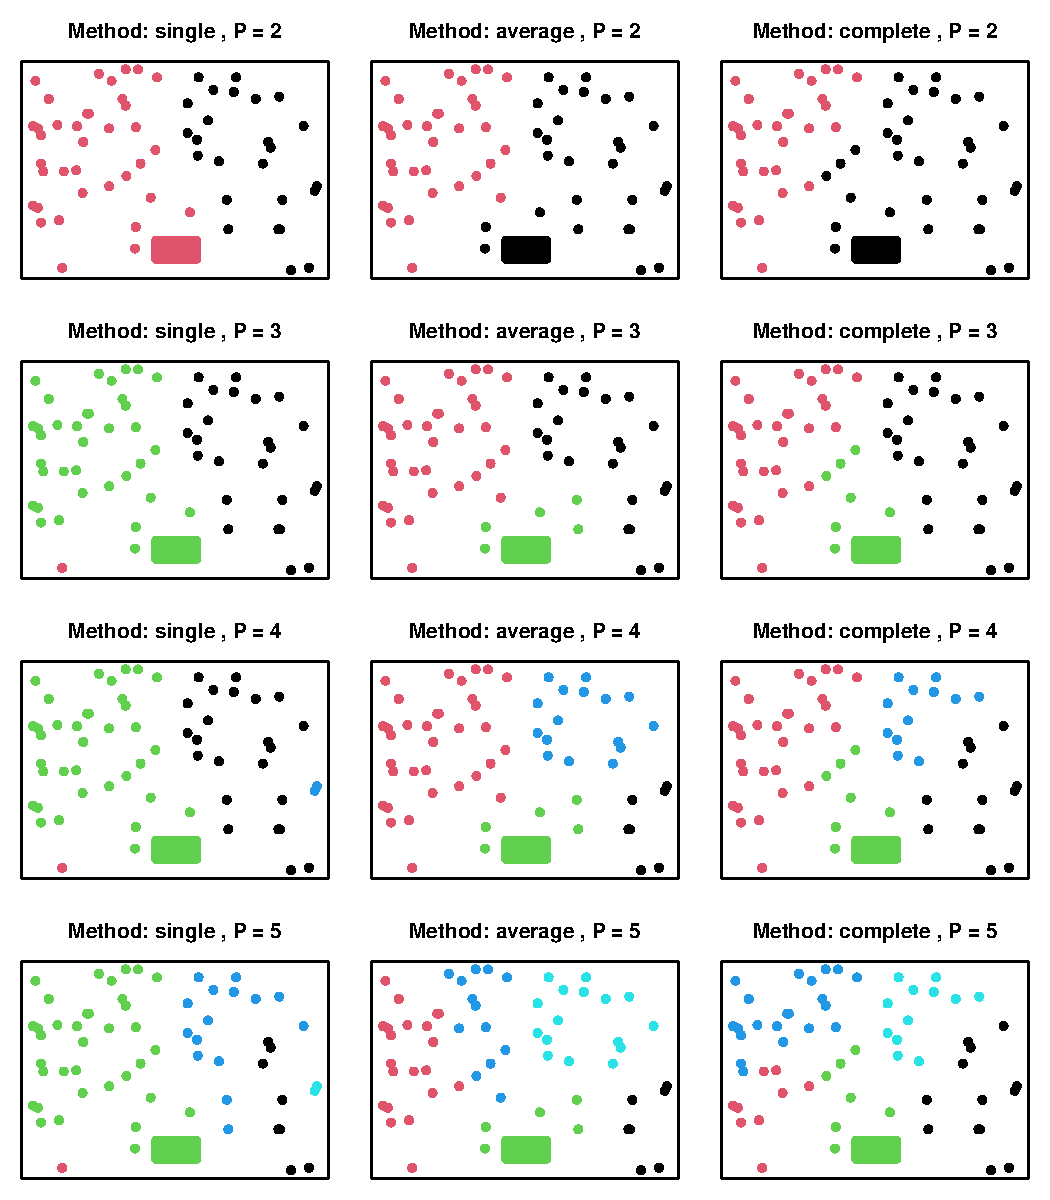
\includegraphics[width = 12cm]{methodsclust.pdf}
	\caption{Example: Different values for P and varying linking methods}
	\label{fig5}
\end{figure}

Coming back to the problem at hand, noise reduction, we would like to exclude as many pixels as possible from the coloured square, i.e., keep the cluster that contains the SRRI shade in tact while removing as many pixels that are obviously not part of the SRRI pixel cloud. Figure 5 gives the impression that complete and average linkage seem to be able to better exclude far off pixels from the SRRI pixel cloud. Further, one can observe that for values p between 2 and 5 the SRRI pixel cloud is not split into multiple clusters, thus a higher value for p is probably advisable. Accuracy comparisons accross different values for p and linking methods will show which combination will yield the best performance.\newpage

\subsubsection{Implementing the AH Clustering Approach}
The function that executes the clustering approach is called \href{https://github.com/Base-R-Best-R/KID/blob/main/Code/Package/KIDs/R/SRRI_ext_loc.R}{\textcolor{teal}{SRRI\_ext\_loc()}}, as inputs it requires the document and the Hex code of the color of the SRRI pixel shade. Additionally, one may choose the linking method as well as the number of final clusters as explained in the previous subsection. The function first slices the bitmap of the document horizontally above and below the scale that is located by \href{https://github.com/Base-R-Best-R/KID/blob/main/Code/Package/KIDs/R/coord_id.R}{\textcolor{teal}{coord\_id()}}. Then using this subset of the original bitmap all pixels in the color of the SRRI shade are extracted and subsequently clustered into groups in order to reduce noise. Next, all groups containing less than a cutoff value of points are discarded to then choose the group with the lowest vertical variance in pixel position as the one being the SRRI shade \citep{datatable}. The idea is that the removal of all pixel groups below a number of points ensures that clusters with very little observations do not end up having the lowest horizontal variance by chance. Alternatively, one could also generate features that describe each of the clusters, such as number of pixels within a cluster, average distance of points within cluster, average variance of vertical and horizontal pixel coordinates to then use predictive methods like decision trees or elastic nets to determin which of the clusters most likely contains the SRRI shade.

\begin{figure}[H]
	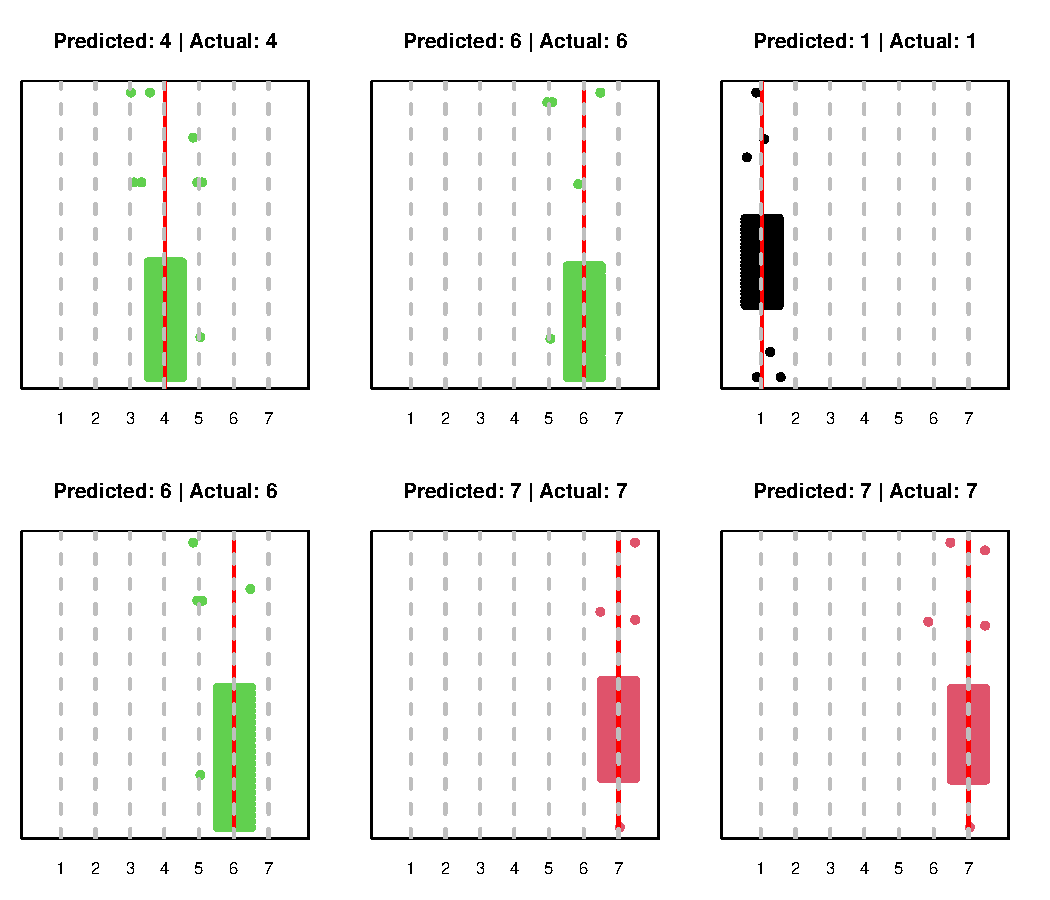
\includegraphics[width = 12cm]{Ersteextr.pdf}
	\caption{SRRI extraction via SRRI\_ext\_loc() using average linkage and $P = 5$}
	\label{fig6}
\end{figure}

 For the actual proccess of clustering the package fastcluster is used, as hierarchichal clustering is not particularly computationally efficient, i.e., depending on the implementation the computational complexity of the algorithm in time is either $\mathcal{O}(n^3)$ or $\mathcal{O}(n^2)$ \citep{JSSv053i09, Rok09}. For ease of imagination a graphical depiction of Erste KID SRRI extraction via \href{https://github.com/Base-R-Best-R/KID/blob/main/Code/Package/KIDs/R/SRRI_ext_loc.R}{\textcolor{teal}{SRRI\_ext\_loc()}} is displayed in figure \ref{fig6}. We observe that the pixel clusters contain very little noise indicating that the function performed as intended.


\section{Parameters and Performance} 
\subsection{In-sample}
The table below summarizes the performance of the extraction in-sample for different parameter choices. Acc. Gross which represents gross accuracy, measures how accurate the extraction is, based on the total number of predicted cases that did not result in an error. This is the most important measure, since the aim is to automize the task of SRRI extraction. Consequently, the worst outcome is an incorrect readout that does not result in an error and is thus undetectable. Usually, one would aspire to have equal or higher gross performance than a human performing the same task, that way the implementation will drastically increase readout speed, when compared to a human and at the same time the amount of errors would be held constant. Of course, in-sample performance is not representative, hence out of sample performance measures are provided in the next section. Acc. net which stands for net performance, tells us how our algorithms performed after accounting for errors. We oberserve that the naive algorithm outperforms the clustering approach significantly. For the optimal in-sample parameters the single-link clustering approach, utilizing four final clusters and tolerance of 20 pixels results in around 12\% less net accuracy.

\begin{table}[H]
	\begin{center}
		\caption{SRRI Classification - In-sample Performance}
		\begin{tabular}{|c|c|c|c|c|c|}
			\hline
			Tolerance & P & Method & Acc. Gross & NA & Acc. Net\\
			\hline
			- & - & naive & 1 & 0.234 & 0.766\\
			\hline
			 20 & 4 & single & 1 & 0.356 & 0.644\\
			\hline
			 20 & 6 & single & 1 & 0.356 & 0.644 \\
			\hline
			 20 & 8 & single & 1 & 0.356 & 0.644 \\
			\hline
			 20 & 4 & average & 1 & 0.356 & 0.644\\
			\hline
			 20 & 6 & average & 1 & 0.356 & 0.644\\
			\hline
			 20 & 4 & complete & 1 & 0.356 & 0.644\\
			\hline
			 20 & 6 & complete & 1 & 0.356 & 0.644\\
			\hline
			 20 & 8 & average & 1 & 0.467 & 0.533\\
			\hline
			 30 & 8 & average & 1 & 0.489 & 0.511\\
			\hline
			 30 & 8 & complete & 1 & 0.500 & 0.500\\
			\hline
		\end{tabular}
	\end{center}
\end{table}

Further, it is also interesting to see that the intuition based on figure \ref{fig5} is apparently incorrect. The linking method seems to be irrelevant as long as the tolerance is low enough. This might be caused by the fact that the amount of far off pixels that the single link tends to generate more frequently do not have enough weight to create incorrectly classifiied cases.

\subsection{Out-of-sample}
Both the naive- as well as the clustering approach, manage to achieve a gross accuracy of 100\%. The net accuracy of the naive method is again drastically higher at 80\%, while the Clustering approach performs slightly better than in-sample at 70\% net accuracy.

\section{Diagnostics and Conclusion}
Now that the accuracy for both approaches is measured, the error sources have to be discussed. In the test sample of 20 KIDs, the 4 documents for which \href{https://github.com/Base-R-Best-R/KID/blob/main/Code/Package/KIDs/R/SRRI_ext_rec.R}{\textcolor{teal}{SRRI\_ext\_rec()}} failed the readout of the SRRI, are all scanned pdfs. Consequently, \href{https://github.com/Base-R-Best-R/KID/blob/main/Code/Package/KIDs/R/coord_id.R}{\textcolor{teal}{coord\_id()}} fails to identify the position of the SRRI graph. Since \href{https://github.com/Base-R-Best-R/KID/blob/main/Code/Package/KIDs/R/SRRI_ext_loc.R}{\textcolor{teal}{SRRI\_ext\_loc()}} utilizes the same helper function, this also explains 20\% of the failed SRRI extractions of the clustering approach. The remaining 10\% are caused by varying colors across different documents, meaning that even though the color of the SRRI shade looks very similar in the documents for the same KAG, the Hex code is actually different. Accordingly, when slicing the bitmap in the extraction proccess the resulting subset is empty. Hence, the required color input is the biggest drawback of the clustering based approach. The reader may rightfully ask, whether this renders the clustering approach obsolete. To an extend it does, for all KIDS that are not scanned the naive approach performs better. However, the clustering approach could in theory allow for the extraction of scanned cases, the idea would be to skip slicing the bitmap above and below the SRRI graph, since localization in scanned pdfs via \href{https://github.com/Base-R-Best-R/KID/blob/main/Code/Package/KIDs/R/coord_id.R}{\textcolor{teal}{coord\_id()}} is built on functionalities of the pdftools package that are not available for scanned files. This approach, does however increase the chances of missclassification as the amount of noise increases drastically and for reasons previously outlined the gross accuracy is the most important performance measure. The implementation of this functionality is beyond the scope of this thesis, however, carefully implemented it could potentially increase the net accuracy while hopefully leaving the gross accuracy at the desired level of 100\%.


%========= Appendix ==========

\appendix


%\section{Code}
%\label{sec:app}

%Appendix for code and additional illustrations

%\subsection{Functions}




%====== References ========
\newpage
\printbibliography


\end{document}
